\documentclass{article}
\usepackage{tikz}
\usetikzlibrary{shapes,arrows,positioning}

\begin{document}

\begin{figure}[h]
\centering
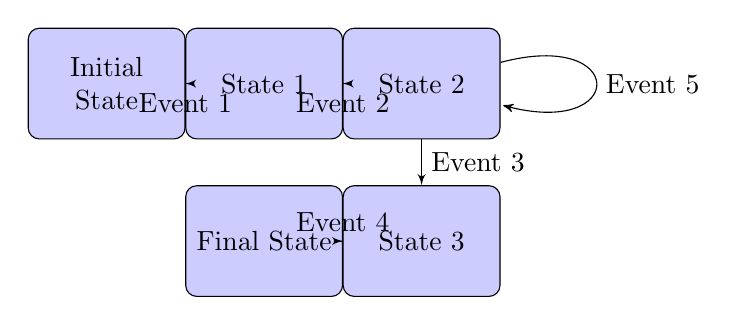
\begin{tikzpicture}[
    node distance=2cm,
    auto,
    >=stealth',
    every node/.style={align=center}
]

% Define styles
\tikzstyle{block} = [rectangle, draw, fill=blue!20, 
    text width=5em, text centered, rounded corners, minimum height=4em]
\tikzstyle{line} = [draw, -latex']

% Nodes
\node [block] (init) {Initial State};
\node [block, right of=init] (state1) {State 1};
\node [block, right of=state1] (state2) {State 2};
\node [block, below of=state2] (state3) {State 3};
\node [block, left of=state3] (final) {Final State};

% Paths
\path [line] (init) -- node {Event 1} (state1);
\path [line] (state1) -- node {Event 2} (state2);
\path [line] (state2) -- node {Event 3} (state3);
\path [line] (state3) -- node {Event 4} (final);

% Self loop
\path [line] (state2) edge [loop right] node {Event 5} ();

\end{tikzpicture}
\caption{Behavior Diagram}
\label{fig:behavior}
\end{figure}

\end{document} 